\chapter{Utilizatori}
\label{chapter:user}

Sistemul de operare oferă resurse pe care utilizatorii să le poată folosi. În
mod obișnuit, utilizatorii creează procese (aplicații) care folosesc resursele
sistemului (procesor, memorie, I/O) pentru a realiza o activitate.
Utilizatorii stochează și transferă date în/din sistemul de calcul, de exemplu
folosind sistemul de fișiere sau rețeaua.

Accesul la un sistem de calcul se realizează prin intermediul unui \textbf{cont de
utilizator} (\textit{user account}). Un utilizator fizic (o persoană) folosește
un cont de utilizator pentru a se identifica în sistem și pentru a folosi resurse cu permisiunile aferente acelui cont de utilizator.
În ceea ce urmează vom folosi, în general, termenul de utilizator ca fiind un
cont de utilizator pe un sistem de calcul.

Sistemele de operare moderne sunt în general multi-utilizator
(\textit{multi-user}), adică permit existența mai multor conturi de utilizator
pe un sistem și rularea simultană a mai multor procese aparținând diferiților
utilizatori. Mai mulți utilizatori pot simultan deschide shelluri locale și rula comenzi
pe un sistem prin conexiuni de rețea la sistem, precum folosind SSH
\abbrev{SSH}{Secure shell}, despre care vom discuta în \labelindexref{Capitolul}{chapter:sec}. Un
cont de utilizator este separat de alt cont astfel că procesele unui utilizator
sunt separate/izolate de procesele altuia, la fel și resursele folosite de procese (precum
fișierele).

Informațiile despre conturile de utilizatori sunt utile nu doar utilizatorilor
avansați, ci și utilizatorilor obișnuiți. Deși utilizatorul obișnuit are în
general un singur cont pe sistemul propriu, informațiile despre conturile de
utilizator îi sunt necesare pentru a înțelege ce acțiuni poate executa pe
sistemul de operare, pentru ce acțiuni are nevoie de accesul la un cont
privilegiat. De asemenea, poate să creeze la nevoie un cont pentru un prieten
sau o rudă pe un sistem al său. Sau se poate autentifica pe sistemul altcuiva și
va trebui să aibă grijă ce informații lasă pe acel sistem. Pentru un utilizator
cu permisiuni speciale (\textit{power user}) sau un administrator,
informațiile despre și operațiile cu utilizatori sunt esențiale pentru a
asigura accesul mai multor utilizatori fizici la un sistem dat, pentru a se
asigura de separarea resurselor între aceștia și între procesele acestora și, în
general, pentru a garanta securitatea sistemului.

Din punctul de vedere al sistemului de operare, un cont de utilizator este
reprezentat de obicei sub forma unui nume de utilizator (\textit{username}).
Acesta este un șir de caractere cu care este identificat utilizatorul. Pentru a
permite accesul în sistem, acestui nume de utilizator i se asociază o formă de
autentificare, precum parolă sau autentificare biometrică. Dacă utilizatorul
fizic furnizează în interfața de acces la sistem un nume de utilizator valid și
forma de autentificare corectă, i se permite accesul în sistem.

Până acum am prezentat conturi de utilizator de sistem, adică acele conturi care
permit crearea de procese și dețin resurse precum fișiere. Există și conturi de
utilizatori de aplicații, precum conturile de utilizatori de aplicații web.
Aceste conturi permit accesul la resurse care sunt gestionate de aplicație, nu
de sistemul de operare. De asemenea, aceste conturi nu permit crearea de procese
sau accesul la resursele sistemului; permit doar accesul gestionat de aplicație
la resursele aplicației.

Indiferent de tipul de cont de utilizator (de sistem sau de aplicație)
principiul de folosire este același: se folosește un nume de utilizator și o
formă de autentificare pentru a permite accesul acestuia la resursele sistemului sau
aplicației. Toate numele de utilizator și formele de autentificare valide sunt
menținute într-o bază de date. Când un utilizator fizic transmite aceste date,
sistemul sau aplicația le verifică dacă sunt prezente în baza de date; în
caz afirmativ se oferă accesul la resurse. Acest mod de folosire este descris în
\labelindexref{Figura}{fig:user:db-access}.

\begin{figure}[htbp]
	\centering
	\def\svgwidth{0.9\columnwidth}
	\includesvg{chapters/05-user/img/acces-bd.svg}
        \caption{Bază de date de access}
        \label{fig:user:db-access}
\end{figure}

În continuare ne vom referi în general la conturile de utilizator de sistem, cu
precizarea că multe concepte se aplică și la conturile de utilizator de
aplicație.

\section{Utilizatori de sistem}
\label{sec:user:system-users}

Așa cum am precizat mai sus conturile de utilizator de sistem sunt folosite
pentru a obține acces la resursele gestionate de sistemul de operare. Conturile
de utilizator permit obținerea unui shell și rularea de comenzi care creează
procese.

De obicei un sistem de operare oferă un prompt grafic sau text de autentificare
unde vor fi completate numele de utilizator și apoi, uzual, parola.

În momentul autentificării unui utilizator de sistem, acesta are acces complet
la o parte din sistemul de fișiere numită \textbf{directorul home al utilizatorului},
reprezentând directorul personal al acestuia. Fiecare sistem de operare are, în
general, un astfel de director pentru utilizatorul de sistem (\file{/home/student} pe
Linux, \file{C:\textbackslash{}Users\textbackslash{}student} pe Windows,
\file{/Users/student} pe macOS). După autentificare, utilizatorul poate crea procese care apoi
accesează fișiere sau alte resurse ale utilizatorului.

\subsection{Permisiuni și privilegii}
\label{sec:user:permissions}

Odată autentificat în sistem, un utilizator are anumite
permisiuni de folosire a sistemului. De exemplu, un utilizator obișnuit poate
crea fișiere doar în directorul său home, dar nu poate instala pachete. Un
alt utilizator poate avea permisiunea de a instala pachete. Sistemul de operare,
pe baza unor configurări, permite unui utilizator anumite acțiuni.

În unele sisteme și aplicații există noțiunea de rol. Un utilizator poate avea
un rol care îi conferă anumite permisiuni. De exemplu, rolul de \texttt{Administrator}
înseamnă, în general, într-o instalare de platformă precum Moodle\footnote{\url{http://www.moodle.org}}, permisiuni complete în cadrul platformei; un rol de
\texttt{Profesor} înseamnă controlul conținutului cursurilor; un rol de
\texttt{Student} înseamnă posibilitatea accesării conținutului.

În general, sistemele oferă anumite permisiuni utilizatorilor.
Structurarea acestor permisiuni este esențială pentru asigurarea securității
sistemului. Dacă un utilizator are mai multe permisiuni decât are nevoie, acesta
va putea abuza sau exploata sistemul. Dacă un atacator din exterior obține
permisiunile unui utilizator (impersonează utilizatorul), pagubele pe care le
provoacă vor fi proporționale cu permisiunile utilizatorului.

Din punctul de vedere al conceptelor de securitate, utilizatorul este un \textbf{agent}
iar resursele puse la dispoziție de sistem sunt \textbf{obiecte}. \textbf{Politica de securitate}
(\textit{security policy}) a sistemului precizează permisiunile și dictează ce
agenți au acces la ce obiecte. În acest context apar adesea termenii de
\textbf{permisiune} și \textbf{privilegiu}.

\begin{definition}{Permisiuni și privilegii}
În general, spunem că permisiunile sunt informații
aferente obiectului care stabilesc ce agenți pot face tipuri de acțiuni, în
vreme ce privilegiile sunt certificate aferente agentului care stabilesc ce
acțiuni poate acesta întreprinde. Mai multe informații găsiți în
\labelindexref{Capitolul}{chapter:sec}.
\end{definition}

În sistemele de operare de uz general (Linux/Unix, Windows, macOS) există, în
general, \textbf{utilizatori obișnuiți} (neprivilegiați) și \textbf{utilizatori privilegiați}.

\begin{definition}{Utilizatori privilegiați și neprivilegiați}
Utilizatorii neprivilegiați au acces complet la o parte din sistemul de fișiere
(directorul home) și pot crea procese care folosesc aceste resurse. Utilizatorii
privilegiați pot face acțiuni care afectează starea globală a sistemului:
instalare de pachete, adăugare/ștergere de utilizatori, repornirea sistemului,
configurarea datei sistemului, schimbarea permisiunilor sistemului, configurarea
rețelei etc.
\end{definition}

În general, există un utilizator al sistemului care are permisiuni complete.
De obicei ne referim la acest utilizator ca \textit{superuser}. Pe sistemele
Linux/Unix este numit \texttt{root}, în vreme ce pe sistemele Windows este numit
\texttt{Administrator}. În multe situații, pentru realizarea unei operații
privilegiate, se accesează contul de \textit{superuser}.

\section{Utilizatorul administrativ (superuser)}
\label{sec:user:superuser}

Utilizatorul administrativ, \textit{superuserul}, deține controlul complet al
sistemului. Toate operațiile privilegiate, inaccesibile unui utilizator obișnuit
neprivilegiat, sunt permise acestuia. Un utilizator obișnuit va accesa acest
cont special (dacă știe parola sau forma de autentificare a acestuia) pentru a
realiza o operație privilegiată.

Faptul că superuserul are acces complet la sistem îl face foarte periculos de
folosit. Dacă un atacator obține acces neautorizat la contul de superuser,
atunci sistemul este compromis. La fel, dacă rulăm greșit o comandă
privilegiată, aceasta poate afecta iremediabil sistemul.

\begin{note}[Comanda rm -fr /]
Comanda \cmd{rm -fr /} este celebră pentru că poate fi folosită pentru a șterge tot sistemul de fișiere. Dacă este folosită de contul de \texttt{root} această comandă șterge conținutul sistemului de fișiere începând de la directorul rădăcină (\texttt{/}). Aveți grijă în folosire acestei comenzi și, ori de câte ori ștergeți un fișier, aveți grijă ce argumente transmiteți comenzii \cmd{rm}.
\end{note}

De aceea, sistemele de operare moderne pun la dispoziția utilizatorul metode de
realizare de acțiuni privilegiate care să nu necesite accesarea directă a
contului privliegiat. Astfel că, în folosirea superuserului, există următoarele
recomandări de folosire:

\begin{itemize}
	\item Să fie folosit contul doar când este absolută nevoie, pentru
		operații privilegiate. Nu vă autentificați ca superuser pe
		interfața grafică.
	\item Să fie o parolă / formă de autentificare cât mai greu de accesat
		în mod neautorizat.
	\item Să fie evitată folosirea superuser-ului când există forme
		alternative de executare de acțiuni privilegiate.
\end{itemize}

Sistemele de operare moderne oferă opțiuni alternative de executare a acțiunilor
privilegiate. În Linux/Unix se poate folosi \cmd{sudo}, bitul setuid, capabilități; le
vom prezenta în \labelindexref{Secțiunea}{sec:user:altroot}.

În Windows, începând cu Windows Vista se folosește \textit{User Account Control}
(UAC\abbrev{UAC}{User Acount Control}), prezentat în \labelindexref{Figura}{fig:user:uac}. \textit{User Account Control} este o tehnologie
care oferă un prompt care trebuie confirmat ori de câte ori se dorește
realizarea unei acțiuni privilegiate. Doar utilizatorilor configurați specific
li se permite rularea de acțiuni privilegiate prin User Account Control.

\begin{figure}[!htbp]
  \centering
  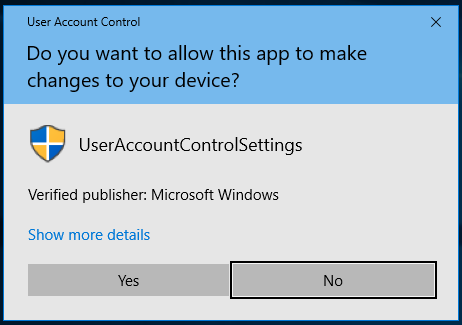
\includegraphics[width=0.6\textwidth]{chapters/05-user/img/uac.png}
  \caption{User Account Control}
  \label{fig:user:uac}
\end{figure}

\subsection{Utilizatorul administrativ în Linux (root)}
\label{sec:user:root}

Utilizatorul administrativ în Linux este numit \texttt{root}. Utilizatorul \texttt{root}
are acces complet la resursele sistemului și poate face orice operații. În
general, accesarea contului de \texttt{root} este evidențiată în linia de comandă prin
prezența simbolului \texttt{\#} (\textit{diez}) în cadrul promptului ca în \labelindexref{Listing}{lst:user:prompt-types}.

\begin{screen}[caption={Prompt neprivilegiat și privilegiat (root)},label={lst:user:prompt-types}]
student@uso:~$ sudo su
[sudo] password for student:
root@uso:/home/student#
\end{screen}

În secvența de mai sus, utilizatorul inițial este \texttt{student}, iar promptul său este marcat de simbolul \texttt{\$} (\textit{dolar}) la finalul promptului. Atunci când folosim comanda \texttt{sudo su} și după ce introducem parola utilizatorului \texttt{student}, obținem un shell privilegiat, marcat de simbolul \texttt{\#} (\textit{diez}) la finalul promptului.

Accesarea unui cont (inclusiv a contului \texttt{root}) se poate face în două moduri:

\begin{itemize}
	\item autentificarea în sistem cu acel cont (la un prompt de login în
		linia de comandă sau în interfața grafică)
	\item schimbarea utilizatorului curent în linia de comandă prin
          folosirea comenzii \cmd{su} (\textit{substitute user})
\end{itemize}

În general, nu este recomandată autentificarea în sistem folosind contul de
\texttt{root}. Orice aplicație care va fi lansată din acest cont va avea acces complet
asupra resurselor sistemului, devenind astfel o posibilă zonă de atac a acestuia.
Este recomandat să folosiți comanda \cmd{su} pentru schimbarea temporară a
utilizatorului și obținerea unui shell de \texttt{root}, folosirea comenzilor
privilegiate și apoi revenirea în consola utilizatorului neprivilegiat folosind
comanda \cmd{exit}, așa cum este ilustrat în \labelindexref{Listing}{lst:user:root-access}.

\begin{screen}[caption={Accesarea contului root},label={lst:user:root-access}]
student@uso:~$ su
Password:
root@uso:/home/student# apt install deluge
[...]
root@uso:/home/student# exit
exit
student@uso:~$
\end{screen}

În \labelindexref{Listing}{lst:user:root-access} am folosind comanda \texttt{su} urmată de introducerea parolei utilizatorului \texttt{root} pentru a accesa contul privilegiat. Acum putem executa acțiuni privilegiate, precum instalarea pachetului \texttt{deluge}. La final folosim comanda \texttt{exit} pentru a încheia sesiunea curentă privilegiată și a reveni la un shell de utilizator neprivilegiat (\texttt{student}).

\subsection{Utilitarul su}
\label{sec:user:su}

Utilitarul \cmd{su} este folosit pentru schimbarea utilizatorului, nu neapărat în
\texttt{root}. Dacă \cmd{su} nu primește nici un argument sau primește ca argument \texttt{root}, va
schimba utilizatorul în \texttt{root}. Altfel va schimba în utilizatorul primit ca
parametru. Așa cum apare în \labelindexref{Listing}{lst:user:su}, la rularea comenzii \cmd{su} se cere parola noului utilizator; fără
introducerea parolei acelui utilizator nu se poate schimba utilizatorul.

\begin{screen}[caption={Schimbarea contului de utilizator folosind comanda su},label={lst:user:su}]
student@uso:~$ su teacher
Password:
teacher@uso:/home/student$ exit
student@uso:~$ su - teacher
Password:
teacher@uso:~$ logout
student@uso:~$ su -l teacher
Password:
teacher@uso:~$ logout
student@uso:~$ su -l teacher -c whoami
Password:
teacher
\end{screen}

Liniile 4 și 7 din \labelindexref{Listing}{lst:user:su} prezintă o formă uzuală de rulare a comenzii \cmd{su} cu opțiunea \texttt{-l} sau \texttt{-}; această formă schimbă mediul de
lucru al viitoarei comenzi, incluzând directorul home. După cum se poate observa, există o diferență între linia \texttt{3} și liniile \texttt{6} și \texttt{9}, care folosesc opțiunile \texttt{-} și \texttt{-l}: după schimbarea utilizatorului se schimbă și directorul curent în directorul home al noului utilizator. Acest lucru se observă în promptul expus de shell.

Utilitarul \cmd{su} permite rularea unei comenzi fără a deschide un shell prin
intermediul opțiunii \texttt{-c}, ca în liniile \texttt{10--12} din \labelindexref{Listing}{lst:user:su}. În felul acesta se rulează direct comanda primită ca
argument și apoi se revine la shell-ul utilizatorului curent, fără a se deschide
un shell al noului utilizator.

\subsection{Alternative la root în Linux}
\label{sec:user:altroot}

Așa cum am precizat anterior, utilizatorul \texttt{root} deține controlul întregului
sistem. Dacă un atacator obține acces neautorizat la contul \texttt{root}, sistemul va fi
compromis. Pe de altă parte, privilegiile pe care le deține utilizatorul \texttt{root}
sunt necesare pentru administrarea sau funcționarea sistemului, precum
configurarea unei interfețe de rețea. De aceea sistemele de operare moderne oferă
opțiuni de granularizare a privilegiilor. În Linux există câteva astfel de
opțiuni printre care amintim bitul setuid, capabilități și utilitarul \cmd{sudo}.

Bitul setuid (\textit{set-user-id-on-execution}) este un bit asociat unui fișier
executabil. Atunci când executăm acel fișier procesul nou creat nu va aparține
utilizatorului care a rulat comanda, ci utilizatorului care deține fișierul, în
mod obișnuit utilizatorul \texttt{root}. \labelindexref{Listing}{lst:user:setuid} conține un exemplu de
folosire a bitului \texttt{setuid}. Observăm în permisiunile fișierelo \texttt{/bin/ping}, \texttt{/bin/su}, \texttt{/usr/bin/sudo} prezența literei \texttt{s}, însemnând bitul setuid.

\begin{screen}[caption={Bitul set-user-id-on-execution (setuid)},label={lst:user:setuid}]
student@uso:~$ ls -l /bin/ping
-rwsr-xr-x 1 root root 64424 Mar 10  2017 /bin/ping
student@uso:~$ ls -l /bin/su
-rwsr-xr-x 1 root root 44664 Jan 25  2018 /bin/su
student@uso:~$ ls -l /usr/bin/sudo
-rwsr-xr-x 1 root root 149080 Jan 31  2020 /usr/bin/sudo
\end{screen}

Prezența bitului \texttt{setuid} pe un executabil deținut de \texttt{root} (de exemplu \cmd{passwd}, \cmd{su},
\cmd{sudo}) înseamnă că acele comenzi pot fi rulate de orice utilizator pentru a crea
procese privilegiate. Vom explica în \labelindexref{Secțiunea}{sec:user:auth}
de ce aceste comenzi sunt privilegiate.

Bitul \texttt{setuid} are dezavantajul că procesul nou creat rulează cu privilegii
complete de \texttt{root}. Dacă acel proces este exploatat, atacatorul va deține un
proces cu permisiuni de \texttt{root} și sistemul va fi compromis. De aceea, pe Linux
există un alt mecanism numit \textbf{capabilități}. Capabilitățile sunt un concept de
bază în sisteme de operare însemnând atașarea unui privilegiu
unui agent (unui obiect). De exemplu, pe sistemele Linux moderne, executabilul
aferent utilitarului ping are atașată capabilitatea \texttt{cap\_net\_raw}. Această
capabilitate înseamnă că procesele create din executabilul \cmd{ping} vor avea
privilegiul de a crea resurse privilegiate necesare utilitarului \cmd{ping}.

Spre deosebire de bitul de setuid, capabilitățile sunt granulare. Privilegiile
aferente contului \texttt{root} sunt separate în capabilități. Un proces are atașate, la
nevoie, doar capabilitățile de care are nevoie; dacă acel proces este exploatat
atunci acțiunile posibile ale atacatorului sunt limitate la ce privilegii oferă
capabilitățile, nu la toate privilegiile contului de \texttt{root}.

Exemple de capabilități pe Linux sunt:

\begin{itemize}
  \item \texttt{cap\_net\_raw}: permite folosirea de sockeți speciali (numiți \textit{raw})
  \item \texttt{cap\_net\_admin}: permite configurarea rețelei
  \item \texttt{cap\_fowner}: permite configurare de permisiuni pe orice fișier
  \item \texttt{cap\_kill}: permite transmiterea de semnale către orice procese
\end{itemize}

\begin{note}[Documentație despre capabilități]
Suportul de capabilități este o componentă avansată a sistemului de
operare, care permite dezvoltatorilor de aplicații configurarea de privilegii
granulare. Pentru mai multe detalii urmăriți pagina de manual, folosind comanda \cmd{man 7 capabilities}.
\end{note}

\subsubsection{Utilitarul sudo}
\label{sec:user:sudo}

Bitul \texttt{setuid} și capabilitățile sunt mecanisme care oferă privilegii unor
executabile și a proceselor pornite din acestea sau, în cazul capabilităților, și mai granular, unor procese. Nu permit ușor atașarea de privilegii unui utilizator
sau configurarea personalizată (\textit{custom}) a acțiunilor care pot fi
executate de acel utilizator. Pentru aceasta, soluția folosită pe sistemele Unix
este \cmd{sudo}.

\cmd{sudo} este un utilitar care permite rularea unor comenzi în numele altui
utilizator, în general \texttt{root}. \cmd{sudo} are o configurare granulară și permite
precizarea explicită a ce comenzi să fie rulate. Spre deosebire de utilitarul
\cmd{su}, la rularea utilitarului \cmd{sudo} nu este nevoie de cunoașterea parolei noului
utilizator, ci a utilizatorului curent.

În mod tipic, când rulăm \cmd{sudo}, îl succedăm cu comanda pe care vrem să o
executăm ca \texttt{root}, ca în exemplele din \labelindexref{Listing}{lst:user:sudo}. Liniile \texttt{1} și \texttt{3} arată rularea unei comenzi în mod privilegiat prin prefixarea acesteia cu \texttt{sudo}.
Adesea dorim obținerea unui shell de \texttt{root} pentru a rula mai multe comenzi
privilegiate. Pentru aceasta rulăm tipic una dintre cele două comenzi de pe liniile \texttt{4--8} din \labelindexref{Listing}{lst:user:sudo}: \texttt{sudo su} sau \texttt{sudo bash}.

\begin{screen}[caption={Folosirea sudo},label={lst:user:sudo}]
student@uso:~$ sudo apt install inkscape
[...]
student@uso:~$ sudo adduser dean
student@uso:~$ sudo su
root@uso:/home/student# exit
student@uso:~$ sudo bash
root@uso:~# exit
student@uso:~$
\end{screen}

Utilitarul \cmd{sudo} permite unui utilizator să ruleze comenzi ca \texttt{root} (sau ca alt
utilizator) printr-o configurație din fișierul de configurare
\file{/etc/sudoers}. \labelindexref{Listing}{lst:user:sudoers} conține secvențe din fișierul de configurare \file{/etc/sudoers}. De exemplu, conform liniei de configurare \texttt{2} utilizatorul \texttt{student} poate rula comenzi ca \texttt{root}.

\begin{screen}[caption={Secvențe din fișierul /etc/sudoers},label={lst:user:sudoers}]
# User privilege specification
student ALL=(ALL:ALL) ALL
teacher ALL=(ALL:ALL) /bin/cat

# Allow members of group admin to execute any command.
%admin  ALL=(ALL) ALL

# Allow members of group sudo to execute any command.
%sudo        ALL=(ALL) ALL
\end{screen}

În mod obișnuit, fișierul \file{/etc/sudoers} are linii de configurare care permit
utilizatorilor din grupul \texttt{admin} sau grupul \cmd{sudo} să poată rula comenzi ca \texttt{root}, precum liniile \texttt{5} și \texttt{9} din \labelindexref{Listing}{lst:user:sudoers}.

În această situație, dacă dorim ca un utilizator să poată rula comenzi ca \texttt{root} îl
adăugăm în grupul admin sau în grupul \cmd{sudo}, nu este nevoie de editarea
fișierului \file{/etc/sudoers}.

\begin{note}[Folosirea contului de root]
E important când e folosit \texttt{root} si când se obține consolă de \texttt{root} și ce
utilizatori au acces la \cmd{sudo}. Avem grijă când acordăm unui utilizator
\textit{permisiuni de sudo}, adică posibilitatea de a rula comenzi ca \texttt{root}, lucru care
poate duce la compromiterea sistemului.
\end{note}

\cmd{sudo} permite configurări mai avansate în fișierul \file{/etc/sudoers}; de exemplu linia
de configurare \texttt{3} din \labelindexref{Listing}{lst:user:sudoers} permite utilizatorului \texttt{teacher} rularea doar a comenzii \texttt{cat}
ca \texttt{root}, permițând vizualizarea tuturor fișierelor din sistem, ca în \labelindexref{Listing}{lst:user:sudo-command}. Utilizatorul \texttt{teacher} nu poate vizualiza conținutul fișierului \file{/etc/sudoers} (folosind comanda \cmd{cat}). Dar poate dacă prefixează cu \texttt{sudo} comanda de afișare.

\begin{screen}[caption={Rularea unei comenzi privilegiate cu sudo},label={lst:user:sudo-command}]
teacher@uso:~$ cat /etc/sudoers
cat: /etc/sudoers: Permission denied
teacher@uso:~$ sudo cat /etc/sudoers
[sudo] password for teacher:
#
# This file MUST be edited with the 'visudo' command as root.
\end{screen}

Fișierul \file{/etc/sudoers} este un fișier important în sistem și de aceea există mai
multe restricții și convenții pentru accesarea acestuia. Astfel, deoarece
configurația sa afectează întreg sistemul de operare, editarea fișierului este
permisă numai utilizatorului privilegiat. De asemenea, pentru a preveni editarea
eronată (ce poate duce sistemul într-o stare de eroare imposibil de rezolvat),
se recomandă folosirea comenzii \cmd{visudo} pentru editare. Pentru editarea sa, fie
rulăm comanda \cmd{visudo} ca \texttt{root}, fie comanda \cmd{sudo visudo}.

\begin{note}[Folosire /etc/sudoers]
Fișierul \file{/etc/sudoers} permite configurări avansate. Puteți parcurge pagina de manual \cmd{man sudoers} sau resursele din Internet\footnote{\url{https://www.digitalocean.com/community/tutorials/how-to-edit-the-sudoers-file-on-ubuntu-and-centos}}.
\end{note}

\paragraph{sudo și redirectare}

O situație frecventă este să redirectăm rezultatul rulării unei comenzi într-un fișier privilegiat (la
care nu avem de obicei acces). De exemplu, dacă dorim să activăm rutarea pe un
sistem Linux, vom rula, ca \texttt{root}, comanda:

\begin{screen}
student@uso:~$ echo 1 > /proc/sys/net/ipv4/ip_forward
\end{screen}

În momentul în care folosim un utilizator neprivilegiat dar care poate folosi \cmd{sudo},
am fi tentați să încercăm să rulăm comanda:

\begin{screen}
student@uso:~$ sudo echo 1 > /proc/sys/net/ipv4/ip_forward
\end{screen}

Acest lucru însă nu funcționează pentru că, deși comanda \cmd{echo 1} rulează ca \texttt{root},
comanda \cmd{sudo}, al cărei output este redirectat, rulează ca utilizator
neprivilegiat. Adică redirectarea cu operatorul \texttt{$>$} are loc pentru comanda \cmd{sudo},
rulată de utilizator neprivilegiat, și nu va reuși.

Soluția la această situație este să nu folosim redirectare ci să folosim o
comandă care primește ca argument acel fișier, iar comanda să ruleze privilegiat
ca \cmd{sudo}. Adică soluția este folosirea comenzii \cmd{tee}, ca mai jos:

\begin{screen}
student@uso:~$ echo 1 | sudo tee /proc/sys/net/ipv4/ip_forward
\end{screen}

În forma de mai sus comanda \cmd{tee} este rulată ca \texttt{root} prin intermediul
utilitarului \cmd{sudo}. Comanda scrie informația primită la intrarea standard (adică
\texttt{1}) în fișierul primit ca argument (\file{/proc/sys/netc/ipv4/ip\_forward}) în mod
privilegiat.

\begin{note}[Folosire \cmd{tee} pentru a scrie într-un fișier privilegiat]
Atunci când dorim să scriem într-un fișier privilegiat fără a accesa o
consolă de \texttt{root}, folosim comanda tee cu \cmd{sudo}. Comanda \cmd{tee} are și opțiunea \texttt{-a}
pentru adăuga informație la sfârșitul fișierului (\textit{append}); în mod obișnuit,
comanda suprascrie conținutul fișierului primit ca argument.
\end{note}

\section{Operații cu utilizatori}
\label{sec:user:operations}

În sistemul de operare un utilizator este reprezentat de procesele și resursele
acestuia. Procesele și resursele (de exemplu fișierele) sunt marcate ca
aparținând utilizatorului.

Pentru un utilizator fizic (o persoană), un utilizator este identificat printr-un
nume de utilizator (\textit{username}); atunci când ne autentificăm, pentru acces folosim
numele de utilizator. La nivelul sistemului de operare, însă, un utilizator este
identificat printr-un număr, numit în mod uzual \textit{user identifier} sau
\textbf{UID}, similar cum un proces este identificat printr-un \textit{process identifier} (PID).

Procesele și fișierele unui utilizator au în atributele acestora câmpul UID.
Pentru procese, acest câmp oferă informații despre ce operații asupra resurselor
sistemului de operare pot fi executate de proces, în timp ce câmpul UID al
fișierelor identifică utilizatorul care le deține. În \labelindexref{Listting}{lst:user:print-uid} afișăm
UID-ul proceselor folosind comanda \cmd{ps} și listăm UID-ul unui fișier folosind
comand \cmd{stat}. Observăm că UID-ul utilizatorului \texttt{student} este \texttt{1000}: liniile \texttt{3}, \texttt{4} și \texttt{9}.

\begin{screen}[caption={Afișare UID pentru procese și fișiere},label={lst:user:print-uid}]
student@uso:~$ ps -o pid,ppid,uid,user,cmd
  PID  PPID   UID USER     CMD
24104 24103  1000 student  -bash
24610 24104  1000 student  ps -o pid,ppid,uid,user,cmd
student@uso:~$ stat vm-actions-log.txt
  File: vm-actions-log.txt
  Size: 4827      	Blocks: 16         IO Block: 4096   regular file
Device: 801h/2049d	Inode: 659107      Links: 1
Access: (0644/-rw-r--r--)  Uid: ( 1000/ student)   Gid: ( 1000/ student)
Access: 2020-08-08 16:32:44.086193999 +0300
Modify: 2018-08-21 14:37:44.316527432 +0300
Change: 2018-08-21 14:37:44.320529432 +0300
 Birth: -
\end{screen}

De obicei, un proces poate avea acces la o resursă dacă UID-ul procesului este
marcat în cadrul resursei ca având acces.

\subsection{Atribute ale utilizatorilor. Informații despre utilizatori}
\label{sec:user:attributes}

Un utilizator are atribute care îi permit identificarea în sistem,
autentificarea și accesul la resurse. Așa cum am precizat mai sus, cele mai
importante două atribute sunt numele de utilizator (\textit{username}) și identificatorul
de utilizator (\textit{user identifier}, UID).

Un utilizator de sistem are acces la un director home (un subdirector în
sistemul de fișiere unde are acces complet). Pentru utilizatorul \texttt{student} acesta
este, în mod uzual, \file{/home/student} (pe Linux), \file{/Users/student} (pe macOS) sau
\file{C:\textbackslash{}Users\textbackslash{}student} (pe Windows).

Pentru autentificare, un utilizator are asociată o parolă sau o altă formă de
autentificare. Aceasta trebuie furnizată la un prompt de login (interfață în
linia de comandă sau grafică) pentru a fi permis accesul în sistem în contul
acelui utilizator.

Pe sistemele Unix, un utilizator are asociat un shell de autentificare (\textit{login
shell}). Este programul care este rulat în momentul autentificării utilizatorului
pe un sistem; programul este, de obicei, un shell în linia de comandă.

Pentru gestiunea mai flexibilă a accesului la resurse, \textbf{utilizatorii sunt
grupați}. Un utilizator face parte din unul sau mai multe grupuri. Astfel că un
administrator care dorește ca mai mulți utilizatori să aibă acces la o anumită
resursă va crea un grup, va adăuga utilizatorii la acel grup și va oferi
grupului permisiuni asupra resursei respective. Un grup poate conține 0 sau mai
mulți utilizatori, iar un utilizator poate aparține unui sau mai multor grupuri,
așa cum este indicat în \labelindexref{Figura}{fig:user:multi-user}.

\begin{figure}[htbp]
	\centering
	\def\svgwidth{\columnwidth}
	\includesvg{chapters/05-user/img/multi-user.svg}
        \caption{Asocierea utilizatori la grupuri}
	\label{fig:user:multi-user}
\end{figure}

De exemplu, în Windows, există grupul \texttt{Administrators}. Un utilizator care este
parte din grupul \texttt{Administrators} are acces complet la sistem.

Aceste atribute sunt definite în fișiere de configurare sau de tip bază de date.
Aceste atribute pot fi, de obicei, vizualizate de orice utilizator, dar
modificate doar de un utilizator privilegiat. Mai multe informații prezentăm în
\labelindexref{Secțiunea}{sec:user:attributes}

\subsection{Obținerea de informații despre utilizatori}
\label{sec:user:user:info}

Informațiile despre utilizatori (nume de utilizator, identificator de
utilizator, director home) pot fi obținute folosind interfețele grafice
aferente unui sistem de operare sau distribuții sau folosind utilitare în linia
de comandă.

În Windows, pentru obținerea de informații despre utilizatori folosim în mod
obișnuit interfața grafică: \textit{Control Panel $\rightarrow$ User Accounts $\rightarrow$ User Accounts}.

\subsubsection{Obținerea de informații despre utilizatori în Linux}
\label{sec:user:linux-user-info}

În Linux, informațiile despre utilizatori sunt stocate în fișiere de configurare
dedicate. În scenarii de administrare mai complexe (care nu fac subiectul
acestei cărți), aceste informații sunt stocate într-o baza de date. Fișierele de
configurare în care sunt reținute informații despre utilizatori sunt indicate în
\labelindexref{Tabelul}{table:user:info-files}.

\begin{table}[!htb]
\caption{Informații despre utilizatori}
\begin{center}
  \begin{tabular}{ p{0.18\textwidth} p{0.22\textwidth} p{0.55\textwidth} }
	\toprule
                \textbf{Fișier} & \textbf{Rol} & \textbf{Informații} \\
	\midrule
                \file{/etc/passwd} & informații utilizatori & nume de utilizator, UID, director home, shell de login, GID \\
	\midrule
                \file{/etc/shadow} & parole utilizatori & nume de utilizator, parolă criptată, informații expirare parolă \\
	\midrule
                \file{/etc/group} & informații grupuri & nume grup, GID, utilizatori aferenți \\
	\bottomrule
	\end{tabular}
        \label{table:user:info-files}
\end{center}
\end{table}

Fișierele de configurare au formă tabelară cu coloane: fiecare linie este o
intrare în tabel iar fiecare coloană este un atribut al acelei intrări. Mai jos
sunt prezentate câteva linii din fiecare fișier de configurare și explicațiile
pentru rolul acestora. Detalii despre fișierele \file{/etc/passwd} și \file{/etc/shadow}
prezentăm în \labelindexref{Secțiunea}{sec:user:auth}.

Putem obține informații despre utilizatori direct din fișierele de configurare
de mai sus, așa cum facem în \labelindexref{Listing}{lst:user:config-files}.

\begin{screen}[caption={Investigarea fișierelor de configurare pentru utilizatori},label={lst:user:config-files}]
student@uso:~$ grep student /etc/passwd
student:x:1000:1000:Student User,,,:/home/student:/bin/bash
student@uso:~$ grep student /etc/group
adm:x:4:syslog,student
cdrom:x:24:student
sudo:x:27:student
dip:x:30:student
plugdev:x:46:student
lpadmin:x:116:student
student:x:1000:
sambashare:x:126:student
student@uso:~$ sudo grep student /etc/shadow
[sudo] password for student:
student:$6$VNq0Dxyc$[...].:17749:0:99999:7:::
\end{screen}

Altfel, informații despre utilizatori obținem folosind utilitare precum cele din
\labelindexref{Tabelul}{table:user:tools-files}. Aceste utilitare investighează fișierele de configurare din \labelindexref{Tabelul}{table:user:info-files}.

\begin{table}[!htb]
\caption{Utilitare de investigare utilizatori}
\begin{center}
  \begin{tabular}{ p{0.20\textwidth} p{0.35\textwidth} p{0.35\textwidth} }
	\toprule
                \textbf{Utilitar} & \textbf{Rol} & \textbf{Fișiere investigate} \\
	\midrule
                \cmd{id} & informații despre utilizator & \file{/etc/passwd}, \file{/etc/group} \\
	\midrule
                \cmd{groups} & grupurile utilizatorului curent & \file{/etc/group} \\
	\midrule
                \cmd{users}, \cmd{w}, \cmd{who} & utilizatorii autentificați în sistem acum & \file{/var/run/utmp} \\
	\midrule
                \cmd{whoami} & numele utilizatorului curent & N/A \\
	\midrule
                \cmd{finger}, \cmd{pinky} & informații complete despre un utilizator & \file{/etc/passwd}, \file{/etc/group} \\
	\bottomrule
	\end{tabular}
        \label{table:user:tools-files}
\end{center}
\end{table}

În \labelindexref{Listing}{lst:user:commands} sunt câteva exemple de folosire ale comenzilor de mai sus.

\begin{screen}[caption={Investigarea utilizatorilor prin comenzi},label={lst:user:commands}]
student@uso:~$ id
uid=1000(student) gid=1000(student) groups=1000(student),4(adm),24(cdrom),27(sudo),30(dip),46(plugdev),116(lpadmin),126(sambashare)
student@uso:~$ id teacher
uid=1001(teacher) gid=1001(teacher) groups=1001(teacher)
student@uso:~$ groups
student adm cdrom sudo dip plugdev lpadmin sambashare
student@uso:~$ groups teacher
teacher : teacher
student@uso:~$ users
student student
student@uso:~$ whoami
student
student@uso:~$ su - teacher -c whoami
Password:
teacher
student@uso:~$ finger
Login     Name           Tty      Idle  Login Time   Office     Office Phone
student   Student User  *:0             Sep  4 17:42 (:0)
student   Student User   pts/0          Sep 19 20:05 (192.168.56.1)
student@uso:~$ finger teacher
Login: teacher        			Name: Teacher User
Directory: /home/teacher            	Shell: /bin/bash
Never logged in.
No mail.
No Plan.
student@uso:~$ pinky
Login    Name                 TTY      Idle   When             Where
student  Student User        ?:0       ?????  2020-09-04 17:42 :0
student  Student User         pts/0           2020-09-19 20:05 192.168.56.1
\end{screen}

În Linux, anumiți utilizatori au configurat ca shell de login \cmd{/bin/false} sau
\cmd{/bin/nologin}. Aceasta înseamnă că acești utilizatori nu se pot autentifica în
sistem și nu pot obține un shell de login. Acești utilizatori mai sunt numiți și
utilizatori de sistem, iar ceilalți sunt numiți utilizatori interactivi.
Utilizatorii de sistem sunt cei care pot avea procese dar nu pot obține shell de
login. Cei interactivi pot obține shell și pot rula apoi comenzi. La o instalare
simplă, o foarte bună parte dintre utilizatorii unui sistem Linux sunt
utilizatori de sistem, așa cum se observă în \labelindexref{Listing}{lst:user:system-users}.

\begin{screen}[caption={Afișarea utilizatorilor de sistem},label={lst:user:system-users}]
student@uso:~$ grep /bin/false /etc/passwd
speech-dispatcher:x:111:29:Speech Dispatcher,,,:/var/run/speech-dispatcher:/bin/false
whoopsie:x:112:117::/nonexistent:/bin/false
hplip:x:118:7:HPLIP system user,,,:/var/run/hplip:/bin/false
gnome-initial-setup:x:120:65534::/run/gnome-initial-setup/:/bin/false
gdm:x:121:125:Gnome Display Manager:/var/lib/gdm3:/bin/false
vboxadd:x:999:1::/var/run/vboxadd:/bin/false

student@uso:~$ grep nologin /etc/passwd
daemon:x:1:1:daemon:/usr/sbin:/usr/sbin/nologin
bin:x:2:2:bin:/bin:/usr/sbin/nologin
sys:x:3:3:sys:/dev:/usr/sbin/nologin
games:x:5:60:games:/usr/games:/usr/sbin/nologin
man:x:6:12:man:/var/cache/man:/usr/sbin/nologin
lp:x:7:7:lp:/var/spool/lpd:/usr/sbin/nologin
[...]
\end{screen}

\subsection{Gestiunea utilizatorilor și grupurilor}
\label{sec:user:groups}

Gestiunea utilizatorilor și grupurilor, însemnând crearea, ștergerea sau
modificarea utilizatorilor și grupurilor poate fi făcută, în mod normal, doar de
un utilizator privilegiat. Operațiile de gestiune a utilizatorilor sunt:

\begin{itemize}
	\item crearea unui utilizator: un nou cont de utilizator, identificat de
          un nume de utilizator (\textit{username}) și un identificator de
		utilizator (UID) este disponibil în sistem
	\item ștergerea unui utilizator: un cont de utilizator este șters din
		sistem, nu mai pot fi create procese cu acest utilizator
	\item crearea unui grup: este creat un grup nou în care pot fi adăugați
		utilizatori
	\item ștergerea unui grup: este șters un grup existent
	\item adăugarea unui utilizator la un grup
	\item ștergerea unui utilizator dintr-un grup
	\item schimbarea parolei unui utilizator
	\item modificarea atributelor unui utilizator: username, login shell,
		director home
\end{itemize}

Aceste operații de gestiune duc la modificarea fișierelor de configurare sau de
tip baze de date din sistem care rețin informațiile despre grupuri și
utilizatori. Operațiile sunt realizate prin utilitare specifice fie din
interfața grafică fie din linie de comandă, ca în \labelindexref{Listing}{lst:user:user-group-linux}.

\subsection{Gestiunea utilizatorilor și grupurilor în Windows}
În Windows, gestiunea utilizatorilor și grupurilor o facem din interfața din
panoul de control. Aceasta este uzual accesibilă din \textit{Control Panel $\rightarrow$ User Accounts $\rightarrow$ User Accounts}, ca în \labelindexref{Figura}{fig:user:windows-users}.

\begin{figure}[!htbp]
	\centering
        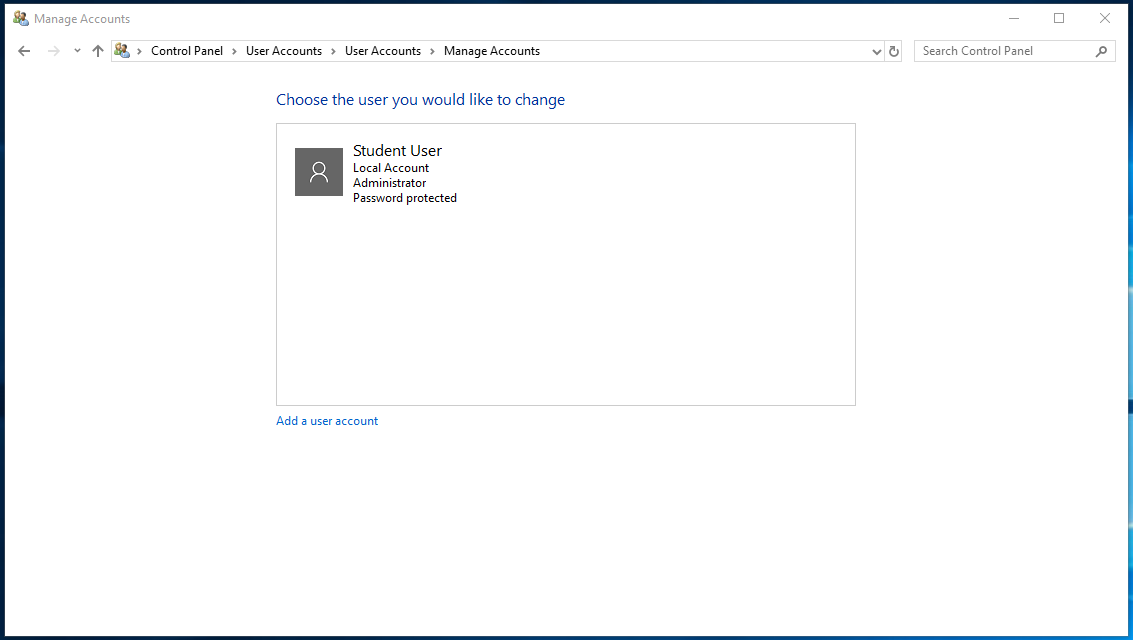
\includegraphics[width=\textwidth]{chapters/05-user/img/windows-user-accounts.png}
        \caption{Gestiunea utilizatorilor în Windows}
        \label{fig:user:windows-users}
\end{figure}

Pe lângă interfața grafică, uzuală, Windows oferă și utilitare în linia de
comandă pentru gestiunea utilizatorilor folosind interfața \cmd{netsh}\footnote{\url{https://docs.microsoft.com/en-us/windows-server/networking/technologies/netsh/netsh-contexts}}.

\subsubsection{Gestiunea utilizatorilor și grupurilor în Linux}
\label{sec:user:user-group-linux}

În Linux există interfețe grafice pentru gestiunea utilizatorilor în funcție de
mediul desktop folosit (GNOME, KDE, XFCE etc.) În mod tradițional, gestiunea se
face în linia de comandă cu ajutorul utilitarelor specifice, indicate în \labelindexref{Tabelul}{table:user:tools-manage}.

\begin{table}[!htb]
\caption{Utilitare de gestiune a utilizatorilor}
\begin{center}
  \begin{tabular}{ p{0.30\textwidth} p{0.20\textwidth} p{0.35\textwidth} }
	\toprule
                \textbf{Operație} & \textbf{Utilitare} & \textbf{Fișiere modificate} \\
	\midrule
                adăugare utilizator & \cmd{useradd} & \file{/etc/passwd}, \file{/etc/shadow}, \file{/etc/group} \\
	\midrule
                ștergere utilizator & \cmd{userdel} & \file{/etc/passwd}, \file{/etc/shadow}, \file{/etc/group} \\
	\midrule
                modificare utilizator & \cmd{usermod} & \file{/etc/passwd}, \file{/etc/shadow}, \file{/etc/group} \\
	\midrule
                adăugare grup & \cmd{groupadd} & \file{/etc/group} \\
	\midrule
                ștergere grup & \cmd{groupdel} & \file{/etc/group} \\
	\midrule
                modificare grup & \cmd{groupmod} & \file{/etc/group} \\
	\midrule
                modificare shell & \cmd{chsh} & \file{/etc/passwd} \\
	\midrule
                modificare informații utilizator & \cmd{chfn} & \file{/etc/passwd} \\
	\midrule
                schimbare parolă & \cmd{passwd} & \file{/etc/shadow} \\
	\bottomrule
	\end{tabular}
        \label{table:user:tools-manage}
\end{center}
\end{table}

Pe distribuțiile bazate pe Debian (Debian, Ubuntu, Linux Mint etc.) există un
set de utilitare mai ușor de folosit care înglobează comenzile de mai sus,
indicate în \labelindexref{Tabelul}{table:user:debian-wrapper}

\begin{table}[!htb]
\caption{Utilitare wrapper Debian}
\begin{center}
  \begin{tabular}{ p{0.40\textwidth} p{0.40\textwidth} }
	\toprule
                \textbf{Utilitar wrapper} & \textbf{Utilitar de bază} \\
	\midrule
                \cmd{adduser} & \cmd{useradd} \\
	\midrule
                \cmd{deluser} & \cmd{userdel} \\
	\midrule
                \cmd{addgroup} & \cmd{groupadd} \\
	\midrule
                \cmd{delgroup} & \cmd{groupdel} \\
	\bottomrule
	\end{tabular}
        \label{table:user:debian-wrapper}
\end{center}
\end{table}

În Linux/Unix există două tipuri de grupuri: \textbf{grupuri primare} și \textbf{grupuri secundare}. Un utilizator
aparține unui singur grup primar și oricâtor grupuri secundare. Când un
utilizator este creat, i se precizează grupul primar aferent. Utilitarul usermod
poate fi folosit pentru modificarea grupurilor din care face parte un utilizator; utilitarul are opțiuni distincte pentru modificarea grupului
primar și pentru modificarea grupurilor secundare.

Un utilizator neprivilegiat are posibilitatea de a-și modifica anumite
informații proprii: shellul de login, numele de utilizator, datele personale,
parola. Pentru aceasta folosește utilitarele din \labelindexref{Tabelul}{table:user:self-manage}.

\begin{table}[!htb]
\caption{Utilitare pentru modificare informații proprii}
\begin{center}
  \begin{tabular}{ p{0.40\textwidth} p{0.40\textwidth} }
	\toprule
                \textbf{Operație} & \textbf{Utilitar} \\
	\midrule
                schimbare shell de login & \cmd{chsh} \\
	\midrule
                schimbare informații & \cmd{chfn} \\
	\midrule
                schimbare parolă & \cmd{passwd} \\
	\bottomrule
	\end{tabular}
        \label{table:user:self-manage}
\end{center}
\end{table}

Un grup care este grupul primar al unui utilizator nu poate fi șters. Întâi trebuie să fie șters utilizatorul, apoi grupul.

În \labelindexref{Listing}{lst:user:user-group-linux} este prezentat un scenariu de lucru cu utilizatori și grupuri în care sunt
folosite comenzile specifice din Linux.

\begin{screen}[caption={Gestiunea utilizatorilor și grupurilor în Linux},label={lst:user:user-group-linux}]
student@uso:~$ sudo groupadd courses
student@uso:~$ sudo adduser teacher courses
Adding user `teacher' to group `courses' ...
Adding user teacher to group courses
Done.
student@uso:~$ users teacher
student@uso:~$ id teacher
uid=1001(teacher) gid=1001(teacher) groups=1001(teacher),1002(courses)
student@uso:~$ sudo adduser george
[...]
student@uso:~$ id george
uid=1002(george) gid=1003(george) groups=1003(george)
student@uso:~$ sudo adduser george courses
Adding user `george' to group `courses' ...
Adding user george to group courses
Done.
student@uso:~$ id george
uid=1002(george) gid=1003(george) groups=1003(george),1002(courses)
student@uso:~$ sudo deluser george courses
Removing user `george' from group `courses' ...
Done.
student@uso:~$ id george
uid=1002(george) gid=1003(george) groups=1003(george)
student@uso:~$ sudo delgroup courses
Removing group `courses' ...
Done.
student@uso:~$ id teacher
uid=1001(teacher) gid=1001(teacher) groups=1001(teacher)
student@uso:~$ sudo deluser george
Removing user `george' ...
Warning: group `george' has no more members.
Done.
student@uso:~$ id george
id: 'george': no such user
\end{screen}

Gestiunea parolelor este o componentă critică a sistemului de operare și o vom
prezenta în secțiunea de mai jos.

\section{Autentificare. Gestiunea parolelor}
\label{sec:user:auth}

Atunci când un utilizator dorește accesul la sistemul de operare trebuie să se
autentifice. Autentificarea presupune, în mod tipic, furnizarea unui nume de
utilizator (\textit{username}) și a unei parole (\textit{password}). Acest lucru este valabil și
pentru aplicații (aplicații web, jocuri, aplicații de baza de date, conturi
bancare). Există și alte moduri de autentificare precum folosirea de informații
biometrice (amprentă digitală, retină), dispozitiv de tip token de
autentificare, autentificare cu cheie publică. În această secțiune vom prezenta
doar autentificarea pe bază de parole.

\subsection{Baza de date de parole}
\label{sec:user:password-db}

Pentru ca autentificarea să reușească, adică utilizatorului să îi fie permis
accesul în sistem, trebuie ca numele de utilizator și parola să fie valide.
Sistemul de operare deține o bază de date cu perechi \textit{(nume de utilizator,
parolă)}. Autentificarea reușește dacă numele de utilizator și parola introduse
de utilizator se găsesc în baza de date.

Baza de date de parole este modificată de acțiunile de lucru cu utilizatori. Adică:

\begin{itemize}
	\item Se adaugă o nouă intrare în baza de date de parole, adică o nouă
          pereche \textit{(nume de utilizator, parolă)} în momentul adăugării unui
		utilizator nou în sistem.
	\item Se șterge o intrare existentă în baza de date de parole în
		momentul ștergerii unui utilizator în sistem.
	\item Se modifică o intrare existentă în baza de date atunci când un
		utilizator își schimbă parola.
\end{itemize}

Baza de date de parole este o componentă critică a sistemului iar accesul la
aceasta trebuie să fie permis numai pentru acțiuni bine definite: autentificare,
adăugarea/ștergerea unui utilizator, schimbarea parolei. Altfel, dacă ar fi
permise și alte acțiuni, un utilizator neprivilegiat ar accesa baza de date și
ar afla parolele altor utilizatori și ar putea folosi conturile acestora, cel
mai periculos fiind folosirea conturilor de utilizatori privilegiați. De aceea,
accesul la baza de date este controlat strict.

Chiar și cu un control strict, se poate întâmpla ca un defect în sistem să
permită unui utilizator neprivilegiat accesul la baza de date de parole. De
aceea parolele nu sunt reținute în format citibil (\textit{plain text}), ci sunt criptate.
Dacă un atacator obține în mod nevalid accesul la baza de date de parole, acesta
va trebui să decripteze parolele, lucru dificil de realizat. Atacuri celebre în
lume au avut ca rezultat obținerea bazelor de date de
parole\footnote{\url{https://en.wikipedia.org/wiki/List\_of\_data\_breaches}}, deci
criptarea acestora e foarte importantă.

În Linux, baza de date de utilizatori este reprezentată de fișierul \file{/etc/passwd}.
Întrucât multe comenzi au nevoie de accesul la acest fișier pentru a obține
UID-ul când se știe numele de utilizator sau pentru a afla shellul
utilizatorului curent, acest fișier nu poate reține parola. Dacă ar fi așa,
orice comenzi uzuale ar putea obține parolele utilizatorilor. Baza de date de
parole este reprezentată în Linux de fișierul \file{/etc/shadow}. Fișierul \file{/etc/shadow}
poate fi accesat doar de utilizatori privilegiați așa cum putem vedea în \labelindexref{Listing}{lst:user:shadow-perm}.

\begin{screen}[caption={Permisiuni de acces pe fișierele de parole},label={lst:user:shadow-perm}]
student@uso:~$ ls -l /etc/passwd
-rw-r--r-- 1 root root 2620 Sep 19 21:08 /etc/passwd
student@uso:~$ ls -l /etc/shadow
-rw-r----- 1 root shadow 1573 Sep 19 21:08 /etc/shadow
\end{screen}

O intrare în fișierul \file{/etc/shadow} conține numele de utilizator, parola criptată
și informații legate de gestiunea parolei, așa cum se observă în \labelindexref{Listing}{lst:user:shadow}.

\begin{screen}[caption={Conținutul fișierului /etc/shadow},label={lst:user:shadow}]
student:$6$VNq0Dxyc$[...].:17749:0:99999:7:::
\end{screen}

Pentru informații detaliate despre formatul intrării și al parolei criptate,
consultați paginile de manual folosind comenzile \cmd{man shadow} și \cmd{man crypt}.

În Windows, baza de date de parole se numește Security Account Manager (SAM
\abbrev{SAM}{Security Account Manager}), și se găsește în
\file{\textbackslash{}\%SystemRoot\%\textbackslash{}system32\textbackslash{}config\textbackslash{}SAM}. Accesul la SAM are loc prin intermediul
Windows Registry și este, similar cu \file{/etc/shadow}, permis numai acțiunilor bine
definite. Similar cu \file{/etc/shadow}, parolele sunt reținute criptate.

\subsection{Gestiunea parolelor}
\label{sec:user:manage-passwords}

Un utilizator își poate gestiona parola proprie, iar un utilizator administrativ
poate gestiona parola tuturor utilizatorilor. Gestiunea parolelor înseamnă în
mod uzual schimbarea lor dar sunt și alte acțiuni. O parolă are asociată o
durată de viață după care expiră; odată expirată, o parolă trebuie să fie
schimbată. Altă acțiune legată de parole este blocarea parolei, astfel încât
autentificarea cu parolă devine inaccesibilă. Sumarizând, există următoarele
acțiuni de gestiune a parolelor:

\begin{itemize}
	\item schimbarea parolei
	\item stabilirea duratei de viață a unei parole
	\item blocarea parolei
\end{itemize}

În Windows se folosește interfața grafică pentru gestiunea parolelor. Se
accesează \textit{Control Panel $\rightarrow$ User Accounts $\rightarrow$ User Accounts $\rightarrow$ Manage Accounts $\rightarrow$ Change an Account $\rightarrow$ Channge password} ca în \labelindexref{Figura}{fig:user:windows-password}.

\begin{figure}[!htbp]
	\centering
        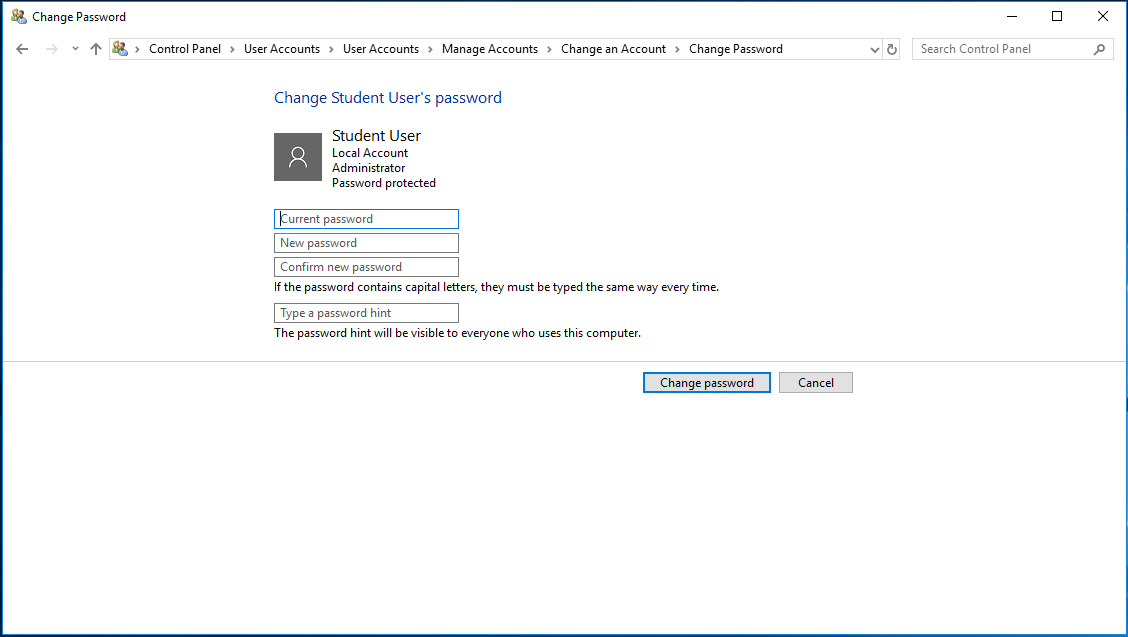
\includegraphics[width=\textwidth]{chapters/05-user/img/windows-password.png}
        \caption{Gestiunea parolelor în Windows}
        \label{fig:user:windows-password}
\end{figure}

În Linux, modul uzual de gestiune a parolei este prin linia de comandă folosind
utilitarul \cmd{passwd}. Cu ajutorul utilitarului \cmd{passwd}, un utilizator neprivilegiat
își poate gestiona parola proprie iar unul privilegiat parola tuturor
utilizatorilor. Atunci când un utilizator neprivilegiat își gestionează parola
folosind utilitarul \cmd{passwd} trebuie să introducă parola la promptul afișat. În \labelindexref{Listing}{lst:user:passwd}
avem exemple de folosire a comenzii \cmd{passwd} pentru gestiunea conturilor.

\begin{screen}[caption={Gestiunea conturilor în Linux folosind passwd},label={lst:user:passwd}]
student@uso:~$ passwd
Changing password for student.
(current) UNIX password:
Enter new UNIX password:
Retype new UNIX password:
passwd: password updated successfully

root@uso:~# passwd teacher
Enter new UNIX password:
Retype new UNIX password:
passwd: password updated successfully
root@uso:~#
\end{screen}

Expirarea parolelor și blocarea parolelor poate fi utilă pentru crearea de
conturi temporare. Cineva primește un cont și apoi nu mai poate să acceseze prin
parolă acel cont pentru că nu mai este parte a unei organizații, are de plătit o
sumă de bani sau altă situație.

De avut în vedere că o parolă blocată nu înseamnă că acel cont nu poate fi
folosit. Un utilizator se poate autentifica la acel cont folosind alte forme de
autentificare, precum autentificare cu chei publice SSH. Dacă dorim să
dezactivăm acel cont și să nu mai poată fi folosit cu nici o formă de
autentificare, putem folosi comanda \cmd{usermod} ca în \labelindexref{Listing}{lst:user:disable}.

\begin{screen}[caption={Dezactivarea unui cont},label={lst:user:disable}]
student@uso:~$ sudo usermod --expiredate 1 teacher
student@uso:~$ su - teacher
Password:
Your account has expired; please contact your system administrator
su: Authentication failure
student@uso:~$
\end{screen}

Comanda configurează contul să expire la \textit{1 ianuarie 1970} făcându-l, astfel,
inutilizabil.

Utilitarul \cmd{passwd} este utilitar interactiv, necesită intrarea de la utilizator.
Ceea ce îl face dificil de folosit pentru automatizare; de exemplu, dacă dorim
să creăm \texttt{100} de conturi pe un sistem cu anumite parole. Pentru aceasta putem
folosi utilitarul \cmd{chpasswd}, ca în \labelindexref{Listing}{lst:user:chpasswd}.

\begin{screen}[caption={Schimbarea neinteractivă a parolei folosind chpasswd},label={lst:user:chpasswd}]
student@uso:~$ echo "teacher:woof2PhaiNiphooS" | sudo chpasswd
\end{screen}

Utilitarul \cmd{chpasswd} primește la intrarea standard linii de forma
\texttt{username:password} și le schimbă în mod neinteractiv, folosibil în scripturi. Mai
sus am schimbat parola utilizatorului \texttt{teacher} la valoarea \texttt{woof2PhaiNiphooS}.

Dincolo de folosirea lor într-un sistem de operare, pentru o persoană, parolele
sunt importante și trebuie avut grijă cum se folosesc. Așa cum vom discuta
detaliat în \labelindexref{Capitolul}{chapter:sec}, folosirea
parolelor poate fi problematică pentru că:

\begin{itemize}
	\item folosim foarte multe parole și, în mod ideal, trebuie să fie
		diferite între ele
	\item parolele pot fi slabe și ușor de ghicit
	\item parolele trebuie să fie schimbate periodic, altfel șansele de fi
		ghicite/decriptate cresc
	\item folosim parolele de pe dispozitive multiple: desktop, laptop,
		dispozitiv mobil
\end{itemize}

Pentru o gestiune corespunzătoare a parolelor există următoarele recomandări:

\begin{itemize}
	\item Parolele să fie lungi (cel puțin 10 caractere) și să conțină
		caractere diferite. Puteți apela la un generator de parole
                precum utilitarul \cmd{pwgen}.
	\item Nu notați parolele în clar pe hârtii sau în fișiere de unde pot fi
		ușor citite.
        \item Folosiți un utilitar de tipul \textit{password manager} care să rețină
		parolele și să minimizeze riscul expunerii lor la un atacator.
		În același timp să ajute să fie accesibile de pe dispozitive
		multiple.
\end{itemize}

\subsection{Autentificare centralizată}
\label{sec:user:centralized-auth}

De multe ori în cadrul unei organizații există mai multe tipuri de aplicații și
interfețe pe care le folosim: un site web, un wiki, un cont Linux, un site
pentru cursuri, un sistem de gestiune a codului sursă. Este problematic pentru
un utilizator să aibă un cont și o parolă diferită pentru fiecare acest tip de
aplicație; utilizatorul poate uita din parole, poate le va nota undeva, sau le
va face simple ca să le țină minte.

Soluția la această situație este autentificarea centralizată. Autentificarea
centralizată presupune existența unui serviciu de autentificare care gestionează
baza de date de parole, serviciu accesat de diferitele aplicații, ca în \labelindexref{Figura}{fig:user:centralized-auth}.

\begin{figure}[htbp]
	\centering
	\def\svgwidth{0.7\columnwidth}
	\includesvg{chapters/05-user/img/auth-central.svg}
        \caption{Autentificare centralizată}
        \label{fig:user:centralized-auth}
\end{figure}

În situația autentificării centralizate, un utilizator folosește același nume de
utilizator și aceeași parolă pentru toate aplicațiile. Aplicațiile trimit mai
departe numele de utilizator și parola către serviciul de autentificare și, dacă
intrările respective sunt valide în baza de date, oferă accesul utilizatorului
la aplicație.

În lumea Windows autentificarea centralizată se bazează pe serviciul AD
\abbrev{AD}{Active Directory} (\textit{Active Directory}) iar în lumea Linux se bazează
pe serviciul LDAP \abbrev{LDAP}{Lightweight Directory Access Protocol}
(\textit{Lightweight Directory Access Protocol}). Aceste subiecte sunt avansate și nu fac
subiectul acestei cărți. Important este înțelegerea nevoii de autentificare
centralizată și principalele soluții pentru asigurarea acesteia.

\section{Accesul la sistemul de fișiere}
\label{sec:user:fs-access}

Conturile de utilizator sunt folosite în sistemul de operare pentru a separa
resursele la care are acces fiecare utilizator. Una dintre cele mai folosite resurse
este sistemul de fișiere; fiecare utilizator dispune de un director home la care
are permisiuni complete.

În general, unui utilizator i se asociază permisiuni pentru o anumită resursă.
De exemplu, utilizatorul \texttt{ana} poate modifica fișierul \file{note.xls} dacă îi sunt
asociate permisiuni de modificare a acelui fișier. La nivel conceptual, un agent
sau un subiect are anumite permisiuni de acces al unei resurse sau un obiect,
așa cum este descris în \labelindexref{Figura}{fig:user:user-file-perm}.

\begin{figure}[htbp]
	\centering
	\def\svgwidth{0.7\columnwidth}
	\includesvg{chapters/05-user/img/agent-perm.svg}
        \caption{Utilizatori, fișiere, permisiuni}
        \label{fig:user:user-file-perm}
\end{figure}

Schema de mai sus este o schemă generală. În cazul particular al secțiunii
curente, agentul este utilizatorul, iar resursa este fișierul. Mai precis,
agentul este un proces aparținând unui utilizator. Spunem că un proces poate
accesa un anumit fișier dacă utilizatorul căruia aparține procesul are
permisiunile aferente la acel fișier.

În multe dintre sistemele de operare moderne, informațiile despre permisiuni sunt reținute în
fiecare fișier. În cadrul fișierului se rețin metadate, printre care și
permisiunile de acces pentru utilizatori. Modul în care sunt structurate aceste
metadate ține de sistemul de operare.

\subsection{Gestiunea permisiunilor în Windows}
\label{sec:user:windows-perm}

În Windows permisiunile sunt reținute în forma unor liste de access (\textit{access
control lists}, ACL \abbrev{ACL}{Access Control Lists}). Adică se creează o listă
de utilizatori sau grupuri de utilizatori și permisiuni aferente, ca în \labelindexref{Figura}{fig:user:acl}.

\begin{figure}[htbp]
	\centering
	\def\svgwidth{0.7\columnwidth}
	\includesvg{chapters/05-user/img/acl.svg}
        \caption{Liste de acces (Windows)}
	\label{fig:user:acl}
\end{figure}

În momentul accesului unui fișier de către un proces, se obține utilizatorul
căruia aparține procesul. Apoi se caută utilizatorul în lista de acces a
fișierului. Dacă există și are asociate permisiuni adecvate, atunci se permite
accesul procesului la fișier. Dacă nu există sau dacă nu are permisiuni, accesul
nu este permis. De obicei în Windows, există o intrare în lista de acces numită
\texttt{Everyone} care precizează permisiunile pentru toți utilizatorii. Dacă, în urma
căutării, un utilizator nu este găsit în listă, atunci se folosesc permisiunile
pentru intrarea \texttt{Everyone}. \labelindexref{Figura}{fig:user:windows-check-perm} verifică modul în care sunt
analizate permisiunile în Windows.

\begin{figure}[htbp]
	\centering
	\def\svgwidth{0.9\columnwidth}
	\includesvg{chapters/05-user/img/check-perm.svg}
	\caption{Verificarea permisiunilor în Windows}
	\label{fig:user:windows-check-perm}
\end{figure}

În Windows permisiunile sunt prezente doar pe sistemul de fișiere NTFS
\abbrev{NTFS}{New Technology File System}, nu și pe FAT32 \abbrev{FAT32}{File
Allocation Table 32}. Permisiunile sunt în mod tipic configurate folosind
interfața grafică: \textit{click dreapta pe fișier $\rightarrow$ Properties $\rightarrow$ Security}, obținând o
fereastră ca cea din \labelindexref{Figura}{fig:user:windows-permissions}.

\begin{figure}[!htbp]
	\centering
        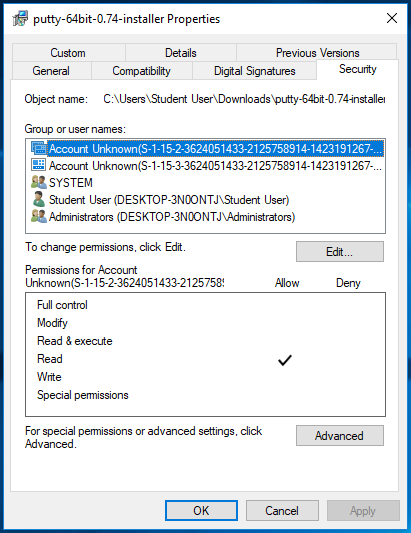
\includegraphics[width=0.5\textwidth]{chapters/05-user/img/windows-permissions.png}
        \caption{Permisiuni în Windows}
        \label{fig:user:windows-permissions}
\end{figure}

Pentru un utilizator dat pot fi precizate mai multe tipuri de permisiuni, dintre
care amintim:

\begin{itemize}
  \item \texttt{List Folder}/\texttt{Read Data}: utilizatorul poate lista conținutul unui
		director și datele unui fișier
  \item \texttt{Create Files}/\texttt{Write Data}: utilizatorul poate crea fișiere într-un
		director și poate scrie date într-un fișier
  \item \texttt{Traverse Folder}/\texttt{Execute File}: utilizatorul poate traversa un
		director și poate executa un fișier
\end{itemize}

Aceste permisiuni sunt similare permisiunilor \texttt{read}, \texttt{write} și \texttt{execute} pe care le
vom prezenta în continuare pentru Linux. O listă completă a permisiunilor în
Windows, pentru NTFS, găsiți pe site-ul care prezintă sistemul de fișiere NTFS\footnote{\url{http://www.ntfs.com/ntfs-permissions-file-folder.htm}}.

\subsection{Gestiunea permisiunilor în Linux}
\label{sec:user:linux-perm}

În Linux fiecare fișiere are metadate. Metadatele relevante pentru permisiuni sunt:

\begin{itemize}
  \item \texttt{user} (utilizator): utilizatorul fișierului
  \item \texttt{group} (grup): grupul fișierului
  \item permisiuni: informații despre ce tipuri accese sunt permise și cui
\end{itemize}

În Linux permisiunile sunt reținute într-un mod simplificat. Există 3 entități
pentru care se pot configura permisiuni și 3 tipuri de permisiuni, ținând cont
de metadatele fișierului. Entitățile sunt:

\begin{itemize}
  \item \texttt{user} (utilizator): utilizatorul fișierului
  \item \texttt{group} (grup): grupul fișierului
  \item \texttt{others} (ceilalți): ceilalți utilizatori, diferiți de utilizatorul
		fișierului și care nu fac parte din grupul fișierului
\end{itemize}

Permisiunile în Linux sunt, de asemenea, simplificate la 3 tipuri:

\begin{itemize}
  \item \texttt{read} (citire): fișierul poate fi citit, directorul poate fi listat
  \item \texttt{item} write (scriere): fișierul poate fi modificat, pot fi adăugate /
		șterse intrări în director
  \item \texttt{execute} (execuție): fișierul poate fi executat, directorul poate
		fi parcurs
\end{itemize}

Permisiunile în Linux sunt verificate în cazul în care un proces accesează un
fișier, urmând pașii:

\begin{enumerate}
	\item Se obține utilizatorul procesului care accesează fișierul.
	\item Se compară utilizatorul procesului cu utilizatorul fișierului.
          Dacă sunt aceiași atunci se obțin permisiunile pentru \texttt{user}
		(utilizator) și se verifică dacă acțiunea procesului este
		acceptată de permisiuni. Dacă da, accesul este permis; dacă nu,
		se trece la pasul următor.
	\item Se obțin toate grupurile din care face parte utilizatorul
		procesului. Se compară, pe rând, fiecare dintre aceste grupuri
		cu grupul fișierului. Dacă există un grup care să corespundă
                grupului fișierului, atunci se obțin permisiunile pentru \texttt{group}
		(grup) și se verifică dacă acțiunea procesului este acceptată de
		permisiuni. Dacă da, accesul este permis; dacă nu, se trece la
		pasul următor.
              \item Se obțin permisiunile pentru \texttt{others} (ceilalți) și se verifică dacă
		acțiunea procesului este acceptată de permisiuni. Dacă da,
		accesul este permis; dacă nu, accesul nu este permis.
\end{enumerate}

Fie următoarea situație de metadate pentru un fișier \file{curs.txt}:

\begin{itemize}
  \item utilizator: \texttt{ana}
  \item grup: \texttt{students}
  \item permisiuni: citire, scriere pentru utilizator, citire pentru grup,
		nici o permisiune pentru ceilalți
\end{itemize}

Utilizatorul \texttt{corina} încearcă accesarea pentru citire a fișierului folosind comanda \cmd{cat curs.txt}. Presupunem că utilizatorul \texttt{corina} aparține mai multor grupuri între care și \texttt{students}, grupul fișierului \file{curs.txt}. Se urmează pașii:

\begin{enumerate}
  \item Se obține utilizatorul procesului care accesează procesul: \texttt{corina}.
  \item Se compară utilizatorul procesului (\texttt{corina}) cu utilizatorul
    fișierului (\texttt{ana}). Nu corespund. Se trece la pasul următor.
  \item Se obțin toate grupurile din care face parte utilizatorul
          procesului (\texttt{corina}). Grupul fișirului \file{curs.txt} este \texttt{students}, grup din care face și utilizatorul \texttt{corina}. În această situație verificăm dacă acțiunea este
		permisă. Acțiunea este de citire, se găsește în permisiunile
                pentru grup (citire), și atunci comanda \cmd{cat curs.txt} reușește.
\end{enumerate}

În situația de mai sus dacă am fi rulat o comandă care modifica fișierul
\file{curs.txt}, nu am fi reușit, pentru că permisiunile pentru grup nu includeau
\textit{scriere}.

Mai jos prezentăm ce permisiuni sunt necesare pentru a putea rula comenzi de
lucru cu sistemul de fișiere:

\begin{itemize}
	\item Pentru a putea traversa un director, pentru ca acesta să fie parte
		a unei căi este suficient ca acesta să aibă permisiuni de
                execuție. Adică dacă dorim să funcționeze comanda \cmd{cd
                /a/b/c/d/}, trebuie ca directoarele \file{a}, \file{b}, \file{c} și \file{d} să aibă
		permisiuni de execuție.
	\item Pentru a putea lista conținutul unui director, adică folosirea
          comenzii \cmd{ls}, trebuie ca acel director să aibă permisiuni de
		citire și de execuție. Pe un director care are doar permisiuni
                de citire nu se poate folosi comanda \cmd{ls}.
	\item Pentru a putea afișa conținutul unui fișier, trebuie ca acel
		fișier să aibă permisiuni de citire iar directorul care-l
		conține să aibă permisiuni de execuție.
	\item Pentru a putea edita un fișier, trebuie ca acel fișier să aibă
		permisiuni de scriere (nu neapărat și de citire) iar directorul
		care-l conține să aibă permisiuni de execuție.
	\item Pentru a putea șterge un fișier sau un director, trebuie ca acel
		fișier sau director să se găsească într-un director care să aibă
		permisiuni de scriere și execuție.
	\item Pentru a putea crea un fișier sau un director, trebuie ca acel
		fișier sau director să fie create într-un director care să aibă
		permisiuni de scriere și execuție.
	\item Pentru a putea rula un fișier executabil, trebuie ca acel fișier
		să aibă permisiuni de citire și execuție iar directorul care-l
		conține să aibă permisiuni de execuție.
\end{itemize}

\subsubsection{Formatul permisiunilor}
\label{sec:user:perm-format}

În mod uzual, permisiunile sunt listate pentru un fișier dat în forma din \labelindexref{Figura}{fig:user:octal-perm}.

\begin{figure}[htbp]
	\centering
	\def\svgwidth{0.7\columnwidth}
	\includesvg{chapters/05-user/img/octal-perm.svg}
        \caption{Permisiuni în Linux}
	\label{fig:user:octal-perm}
\end{figure}

Adică permisiunile sunt listate ca un șir de nouă caractere:

\begin{itemize}
  \item primele trei caractere sunt permisiunile pentru \texttt{user} (utilizator)
  \item următoarele trei caractere sunt permisiunile pentru \texttt{group} (grup)
  \item ultimele trei caractere sunt permisiunile pentru \texttt{others} (ceilalți)
\end{itemize}

\begin{screen}[caption={Listare permisiuni pe fișiere},label={lst:user:list-perm}]
student@uso:~$ ls -l invoice.pdf
-rw-rw-r-- 1 dan staff 0 Sep 19 21:40 invoice.pdf
student@uso:~$ ls -l export_grades
-rwxr-x--- 1 dan adm 0 Sep 19 21:41 export_grades
student@uso:~$ stat invoice.pdf
  File: invoice.pdf
  Size: 0         	Blocks: 0          IO Block: 4096   regular empty file
Device: 801h/2049d	Inode: 658479      Links: 1
Access: (0664/-rw-rw-r--)  Uid: ( 1002/     dan)   Gid: (   50/   staff)
Access: 2020-09-19 21:40:40.242001000 +0300
Modify: 2020-09-19 21:40:40.242001000 +0300
Change: 2020-09-19 21:41:55.110001000 +0300
 Birth: -
student@uso:~$ stat export_grades
  File: export_grades
  Size: 0         	Blocks: 0          IO Block: 4096   regular empty file
Device: 801h/2049d	Inode: 683312      Links: 1
Access: (0750/-rwxr-x---)  Uid: ( 1002/     dan)   Gid: (    4/     adm)
Access: 2020-09-19 21:41:26.414001000 +0300
Modify: 2020-09-19 21:41:26.414001000 +0300
Change: 2020-09-19 21:42:00.170001000 +0300
 Birth: -
\end{screen}

Astfel, în \labelindexref{Listing}{lst:user:list-perm} avem următoarele:

\begin{itemize}
  \item fișierul \file{invoice.pdf} are:
	\begin{itemize}
          \item permisiuni de citire și scriere pentru \texttt{user}, adică pentru
                  utilizatorul \texttt{dan}
                \item permisiuni de citire și scriere pentru \texttt{group}, adică pentru
                  grupul \texttt{staff}
		\item permisiuni de citire pentru ceilalți
	\end{itemize}
  \item fișierul \file{export_grades} are:
	\begin{itemize}
          \item permisiuni de citire, scriere și execuție pentru \texttt{user},
                  adică pentru utilizatorul \texttt{dan}
                \item permisiuni de citire și execuție pentru \texttt{group}, adică
                  pentru grupul \texttt{adm}
	\end{itemize}
	\item nici o permisiune pentru ceilalți
\end{itemize}

Pentru gestiunea mai rapidă a permisiunilor acestea sunt gestionate în format pe
biți. Adică fiecare dintre cele nouă caractere de permisiuni ocupă un bit; bitul
este 1 dacă permisiunea este activă și pe 0 dacă este inactivă. Adică avem
corespondențe de forma:

\begin{itemize}
  \item \texttt{rw-r-{}-r-{}-} corespunde \texttt{110100100}
  \item \texttt{rwxr-x-{}-{}-} corespunde \texttt{111101000}
  \item \texttt{rw-rw-{}-{}-{}-} corespunde \texttt{110110000}
\end{itemize}

Pentru a fi mai rapid, grupurile de biți se grupează câte trei (trei biți pentru \texttt{user},
trei biți pentru \texttt{group}, trei biți pentru \texttt{others}) și cei trei biți se transformă într-o
cifră în octal (baza 8); de aceea mai numim reprezentarea octală. Avem, așadar,
corespondența:

\begin{itemize}
  \item \texttt{rw-r-{}-r-{}-} corespunde \texttt{110100100}, adică \texttt{644} în octal
  \item \texttt{rwxr-x-{}-{}-} corespunde \texttt{111101000}, adică \texttt{750} în octal
  \item \texttt{rw-rw-{}-{}-{}-} corespunde \texttt{110110000}, adică \texttt{660} în octal
\end{itemize}

Pentru că este ușor de modificat și rapid de folosit, gestiunea permisiunilor
se face, adesea, în format octal.

\subsection{Comenzi pentru gestiunea permisiunilor}
\label{sec:user:perm-cmd}

Pentru gestiunea permisiunilor avem comenzi de afișare a metadatelor de
fișierului (utilizator, grup și permisiuni) și comenzi de modificare a
metadatelor.

Pentru afișarea metadatelor, cele două comenzi folosite sunt \cmd{ls -l} și \cmd{stat}
ca în \labelindexref{Listing}{lst:user:list-perm}. În rezultatul rulării comenzilor avem utilizatorul, grupul și permisiunile.

Comenzile de modificare sunt \cmd{chown}, \cmd{chgrp} și \cmd{chmod}. Primele două comenzi (\cmd{chown}
și \cmd{chgrp}) modifică utilizatorul și grupul, iar \cmd{chmod} modifică permisiunile. Comanda
\cmd{chown} poate modifica și utilizatorul și grupul unui fișier, comanda \cmd{chgrp} doar
grupul. Cele două comenzi pot fi rulate doar de utilizatorul privilegiat; doar
acesta poate modifica utilizatorul și grupul unui fișier. \labelindexref{Listing}{lst:user:chown} conține exemple
de folosire a comenzilor \cmd{chown} și \cmd{chgrp}.

\begin{screen}[caption={Modificarea utilizatorului și grupului unui fișier},label={lst:user:chown}]
student@uso:~$ ls -l  invoice.pdf
-rw-rw-r-- 1 dan staff 0 Sep 19 21:40 invoice.pdf
student@uso:~$ sudo chown student invoice.pdf
student@uso:~$ ls -l  invoice.pdf
-rw-rw-r-- 1 student staff 0 Sep 19 21:40 invoice.pdf
student@uso:~$ sudo chown teacher:gdm invoice.pdf
student@uso:~$ ls -l invoice.pdf
-rw-rw-r-- 1 teacher gdm 0 Sep 19 21:40 invoice.pdf
student@uso:~$ sudo chgrp avahi invoice.pdf
student@uso:~$ ls -l invoice.pdf
-rw-rw-r-- 1 teacher avahi 0 Sep 19 21:40 invoice.pdf
\end{screen}

Comanda \cmd{chmod} modifică permisiunile fișierelor. Comanda poate fi rulată de
utilizatorul privilegiat sau de cel ce deține fișierul (\textit{owner}), adică
utilizatorul fișierului; altfel spus, un utilizator își poate modifica
permisiunile fișierelor proprii. Comanda de modificare primește o construcție de
modificare a permisiunilor și numele fișierului/fișierelor pentru care dorim
schimbarea permisiunilor. \labelindexref{Listing}{lst:user:chmod} conține exemple
de folosire a comenzii \cmd{chmod}:

\begin{screen}[caption={Modificarea permisiunilor unui fișîer},label={lst:user:chmod}]
student@uso:~$ ls -l road-trip.png
-rw-rw-r-- 1 student student 0 Sep 19 21:47 road-trip.png
student@uso:~$ chmod g-w,o+w road-trip.png
student@uso:~$ ls -l road-trip.png
-rw-r--rw- 1 student student 0 Sep 19 21:47 road-trip.png
student@uso:~$ chmod a-r road-trip.png
student@uso:~$ ls -l road-trip.png
--w-----w- 1 student student 0 Sep 19 21:47 road-trip.png
student@uso:~$ chmod u=rw,g=r,o= road-trip.png
student@uso:~$ ls -l road-trip.png
-rw-r----- 1 student student 0 Sep 19 21:47 road-trip.png
student@uso:~$ chmod 644 road-trip.png
student@uso:~$ ls -l road-trip.png
-rw-r--r-- 1 student student 0 Sep 19 21:47 road-trip.png
\end{screen}

Forma în octal a permisiunilor la \cmd{chmod} este preferată atunci când vrem să
configurăm un nou set de permisiuni unui fișier. Când vrem să actualizăm
permisiunile și modificările sunt mici, este de preferat să folosim forma în
octal a permisiunilor.

\subsubsection{Permisiuni de creare pentru fișiere}
\label{sec:user:umask}

Atunci când creăm un fișier sau director, folosind, de exemplu, comenzile \cmd{touch}
și \cmd{mkdir}, le sunt asociate metadate implicite la creare. Utilizatorul și grupul
fișierului vor fi utilizatorul și grupul procesului, care sunt, de obicei,
utilizatorul și grupul primar al utilizatorului care a lansat comanda.
Stabilirea permisiunilor la creare ține de \textbf{masca de creare a shellului} (numită și \texttt{umask}).

Masca de creare a shellului este o valoare pe biți care este folosită astfel:

\begin{itemize}
  \item Pentru fișiere se face un \textbf{ȘI logic} între valoarea \texttt{666} (octal) și
		masca inversată.
  \item Pentru directoare se face un \textbf{ȘI logic} între valoarea \texttt{777} (octal)
		și masca inversată.
\end{itemize}

Deosebirea între fișiere și directoare apare pentru că directoarele au nevoie de permisiuni de execuție pentru
toate operațiile. Iar fișierele nu au nevoie de permisiuni de execuție; dacă
este cazul acestea trebuie acordate explicit.

Exemple sunt prezente în \labelindexref{Tabelul}{table:user:umask}.

\begin{table}[!htb]
\caption{Permisiuni de creare fișier în funcție de mască}
\begin{center}
  \begin{tabular}{ p{0.20\textwidth} p{0.20\textwidth} p{0.20\textwidth} p{0.20\textwidth} }
	\toprule
                \textbf{Mască de creare} & \textbf{Mască inversată} & \textbf{Permisiuni de creare fișier} & \textbf{Permisiuni de creare director} \\
	\midrule
                \texttt{022} & \texttt{755} & \texttt{644} & \texttt{755} \\
	\midrule
                \texttt{002} & \texttt{775} & \texttt{664} & \texttt{775} \\
	\midrule
                \texttt{077} & \texttt{700} & \texttt{600} & \texttt{700} \\
	\bottomrule
	\end{tabular}
        \label{table:user:umask}
\end{center}
\end{table}

Afișarea și modificarea măștii shellului se face folosind comanda \cmd{umask}. Fără
parametru această comandă afișează masca de creare, iar cu parametru modifică
masca de creare, ca în \labelindexref{Listing}{lst:user:umask}.

\begin{screen}[caption={Masca de creare a fișirelor (umask)},label={lst:user:umask}]
student@uso:~$ umask
0002
student@uso:~$ touch ana.txt
student@uso:~$ ls -l ana.txt
-rw-rw-r-- 1 student student 0 Sep 19 21:50 ana.txt
student@uso:~$ mkdir bogdan.dir
student@uso:~$ ls -ld bogdan.dir
drwxrwxr-x 2 student student 4096 Sep 19 21:50 bogdan.dir
student@uso:~$ umask 0022
student@uso:~$ umask
0022
student@uso:~$ touch corina.txt
student@uso:~$ ls -l corina.txt
-rw-r--r-- 1 student student 0 Sep 19 21:51 corina.txt
student@uso:~$ mkdir dan.dir
student@uso:~$ ls -ld dan.dir
drwxr-xr-x 2 student student 4096 Sep 19 21:51 dan.dir
\end{screen}

Tot în \labelindexref{Listing}{lst:user:umask} (liniile \texttt{9--17}) sunt exemple de modificare a umask-ului și crearea de fișiere și
directoare pentru a vedea cum modificarea valorii umask duce la modificarea
măștii de creare a shellului și, astfel, a permisiunilor de creare pentru
fișiere și directoare.

\subsection{Biți speciali de acces: setuid, setgid, sticky}
\label{sec:user:special-bits}

Atunci când afișăm masca de creare a shell-ului, observăm că sunt patru cifre octale
afișate. În mod normal ar trebui să fie trei cifre afișate, cu permisiuni pentru
\texttt{user}, \texttt{group} și \texttt{others}. Prima cifră afișată reprezintă un set special de trei de
biți numiți \texttt{setuid}, \texttt{setgid} și \texttt{sticky}, și sunt activați în această ordine.
Astfel, pentru permisiunile de mai jos avem explicațiile:

\begin{itemize}
  \item \texttt{4755}: este activat bitul \texttt{setuid}, utilizatorul are permisiuni
		complete, grupul are permisiuni de citire și execuție, ceilalți
		au permisiuni de citire și execuție
              \item \texttt{2755}: este activat bitut \texttt{setgid}, celelalte permisiuni sunt ca mai
		sus
              \item \texttt{1755}: este activat bitul \texttt{sticky}, celelalte permisiuni rămân la fel
\end{itemize}

Bitul \texttt{setuid} are sens când este folosit pe fișiere executabile. Adaugă
funcționalitatea de set user ID on execution. Când un fișier executabil are
activat bitul \texttt{setuid}, procesul creat din acest fișier executabil va avea
utilizatorul ale acestui fișier (de obicei \texttt{root}) nu al utilizatorului care a
rulat comanda. Mai concret, dacă rulăm ca utilizator \texttt{student} executabilul \cmd{myexec}
care are activat bitul \texttt{setuid} și are ca utilizator \texttt{root}, atunci procesul creat
din executabilul \cmd{myexec} va rula ca utilizatorul \texttt{root}.

Bitul \texttt{setuid}, prezentat și în \labelindexref{Secțiunea}{sec:user:altroot} este folosit atunci când anumite utilitare necesită privilegii
pentru accesarea unor fișiere speciale atunci când rulează. În \labelindexref{Listing}{lst:user:use-setuid},
executabilul \file{/usr/bin/passwd} are activat bitul setuid pentru că procesul creat
va trebui să acceseze fișierul \file{/etc/shadow}, fișier accesibil doar utilizatorilor
privilegiați.

\begin{screen}[caption={Folosirea bitului setuid},label={lst:user:use-setuid}]
student@uso:~$ ls -l /usr/bin/passwd
-rwsr-xr-x 1 root root 59640 Jan 25  2018 /usr/bin/passwd
student@uso:~$ stat /usr/bin/passwd
  File: /usr/bin/passwd
  Size: 59640             Blocks: 120        IO Block: 4096   regular file
Device: 801h/2049d        Inode: 656195      Links: 1
Access: (4755/-rwsr-xr-x)  Uid: (    0/    root)   Gid: (    0/    root)
Access: 2018-08-21 11:41:23.741306286 +0300
Modify: 2018-01-25 17:09:22.000000000 +0200
Change: 2018-08-06 17:34:29.848000000 +0300
 Birth: -
\end{screen}

Vedem în rezultatul rulării comenzilor prezența cifrei \texttt{4} pe prima poziție în forma octală a
permisiunilor și a caracterului \texttt{s} în forma literală a permisiunilor în locul
caracterului de execuție pentru utilizator. Aceasta înseamnă prezența bitului \texttt{setuid} în permisiunile fișierului.

Bitul \texttt{setgid} are sens când este folosit pe executabile și pe directoare. Adaugă
funcționalitatea de \textit{set group ID on execution}. Pe executabile are
același efect ca bitul \texttt{setuid} doar că pentru grup.

Când un director are activat bitul \texttt{setgid}, viitoarele subdirectoare și fișiere ale
acestuia vor avea ca grup în metadate grupul directorului, nu grupul
utilizatorului care a rulat comanda. Viitoarele subdirectoare vor moșteni bitul
\texttt{setgid} astfel că ce se creează nou în ierarhie va avea mereu același grup. Este
util pentru a crea un spațiu partajat în care diferiți utilizatori să creeze
fișiere dar să rămână accesibile între ei câtă vreme fac parte din același grup.
Mai concret, dacă directorul \file{top/} are grupul \texttt{heroes} și are activat bitul
\texttt{setgid}, viitoarele fișiere și subdirectoare vor avea tot grupul \texttt{heroes},
indiferent ce utilizatori au creat intrările.

\labelindexref{Listing}{lst:user:setgid} prezintă cum activarea bitului \texttt{setgid} pe un director duce
la crearea de intrări care moștenesc grupul directorului.

\begin{screen}[caption={Folosirea bitului setgid},label={lst:user:setgid}]
student@uso:~$ ls -ld top/
drwxr-xr-x 2 student heroes 4096 Sep 19 21:54 top/
student@uso:~$ sudo chmod g+s top/
student@uso:~$ ls -ld top/
drwxr-sr-x 2 student heroes 4096 Sep 19 21:54 top/
student@uso:~$ mkdir top/alamar
student@uso:~$ ls -ld top/alamar
drwxr-sr-x 2 student heroes 4096 Sep 19 21:55 top/alamar
\end{screen}

Bitul \texttt{sticky} are sens când este folosit pe directoare la care au acces de
scriere mai mulți utilizatori, de exemplu directorul \file{/tmp}. Adaugă
funcționalitatea de \textit{restricted deletion flag}. Acest lucru înseamnă că un
utilizator nu poate șterge fișierele altui utilizator, deși are permisiuni de
scriere pe directorul care conține acele fișiere.

Directorul \file{/tmp} este cel care are activat bitul \texttt{sticky} pentru că oferă
permisiuni complete tuturor utilizatorilor. Deși un utilizator are permisiuni
complete pe acel director, nu poate șterge fișiere care nu-i aparțin, așa cum
avem prezentat în \labelindexref{Listing}{lst:user:sticky}.

\begin{screen}[caption={Folosirea bitului sticky},label={lst:user:sticky}]
student@uso:~$ ls -ld /tmp/
drwxrwxrwt 13 root root 4096 Sep 19 21:54 /tmp/
\end{screen}

\section{Anexă: Resetarea parolei în Linux}
\label{sec:user:linux-password-recovery}

Se poate întâmpla să fie uitată parola administrativă pe un sistem care rulează
Linux. În această situație este nevoie de resetarea parolei contului \texttt{root}.
Pentru aceasta avem două opțiuni:

\begin{itemize}
	\item modificarea procesului de boot și înlocuirea procesului init
	\item folosirea unui stick USB \abbrev{USB}{Universal Serial Bus} sau CD
		bootabil
\end{itemize}

Procesul de boot va fi prezentat detaliat în \labelindexref{Capitolul}{chapter:boot}.

În prima variantă, în ecranul bootloader-ului GRUB \abbrev{GRUB}{GRand Unified
Bootloader} edităm linia de boot și
adăugăm șirul \texttt{init=/bin/bash}, ca în \labelindexref{Figura}{fig:user:grub-init-bash}.

\begin{figure}[!htbp]
  \centering
  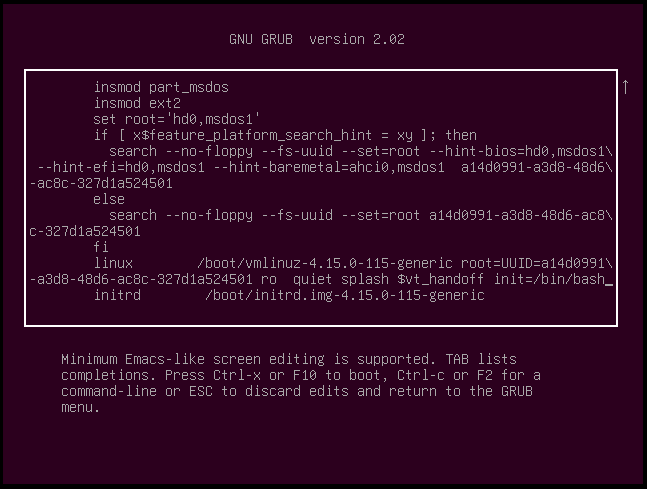
\includegraphics[width=0.8\textwidth]{chapters/05-user/img/grub-init-bash.png}
  \caption{Pornirea în shell privilegiat din GRUB}
  \label{fig:user:grub-init-bash}
\end{figure}

Apoi folosim combinația de taste \texttt{Ctrl+x} pentru a boota sistemul de operare. În
această situație primul proces pornit de sistem nu va fi init ci va fi un shell
cu permisiuni de \texttt{root}. În acest shell vom rula comenzile din \labelindexref{Listing}{lst:user:change-root-pw} pentru
schimbarea parolei utilizatorului \texttt{root}.

\begin{screen}[caption={Schimbarea parolei contului root în shell-ul privilegiat},label={lst:user:change-root-pw}]
root@none:~# mount -o remount /
root@none:~# passwd
[...]
\end{screen}

Mai sus am folosit comanda mount pentru a remonta sistemul de fișiere rădăcină
în modul \textit{read-write} și a putea astfel modifica fișierul \file{/etc/shadow} cu ajutorul
comenzii \cmd{passwd}.

Apoi repornim sistemul fie din buton, fie folosind combinația de taste
\texttt{Ctrl+Alt+Del}. Nu vom putea folosi comenzi precum \cmd{reboot} sau \cmd{poweroff}.

În a doua variantă, folosim un CD/stick USB bootabil cu o distribuție Linux live
(precum Ubuntu). După ce sistemul va porni distribuția live, vom realiza
următorii pași:

\begin{enumerate}
  \item Montăm sistemul de fișiere rădăcină al sistemului Linux instalat
		(pentru care vrem să resetăm parola contului \texttt{root}).
  \item Folosim comanda \cmd{chroot} pentru a modifica sistemul de fișiere
		rădăcină în care rulăm în sistemul de fișiere al sistemului
		Linux instalat
  \item Folosim comanda \cmd{passwd} pentru a schimba parola contului \texttt{root} în
		sistemul de fișiere rădăcină al sistemului Linux instalat.
  \item Revenim la sistemul de fișiere al sistemului live, părăsind
        shell-ul obținut prin \cmd{chroot}.
  \item Demontăm sistemul de fișiere rădăcină al sistemului Linux
		instalat.
  \item Repornim sistemul.
\end{enumerate}

Pașii de mai sus sunt reproduși în comenzile din \labelindexref{Listing}{lst:user:pw-reset-live-cd}.

\begin{screen}[caption={Resetarea parolei contului root cu live CD},label={lst:user:pw-reset-live-cd}]
root@ubuntu:~# mkdir /mnt/rootfs
root@ubuntu:~# mount /dev/sda1 /mnt/rootfs
root@ubuntu:~# chroot /mnt/rootfs
root@ubuntu:~# passwd
[...]
\end{screen}

\section{Use case: Resetarea parolei în Windows}
\label{sec:user:windows-password-recovery}

Pentru resetarea parolei unui utilizator în Windows, cel mai important fiind
utilizatorul \texttt{Administrator}, se poate folosi utilitarul \cmd{chntpw} (de la change NT
password). Acesta este inclus în mai multe CD-uri de recuperare (rescue CDs).

O opțiune este folosirea Ultimate Boot
CD\footnote{\url{http://www.ultimatebootcd.com}}, un CD bootabil cu utilitare
diverse de diagnostic și reparație la nivelul sistemului de operare. Ultimate
Boot CD conține PartedMagic\footnote{\url{https://partedmagic.com}} care, la
rândul său, conține utilitarul \cmd{chntpw}. Utilitarul \cmd{chntpw} oferă interfață în
linia de comandă pentru modificarea parolelor utilizatorilor în Windows.

Pentru a nu ocupa spațiu din această carte cu detalii, recomandăm să parcurgeți
tutorialul cu screenshot-uri despre folosirea Ultimate Boot CD pentru resetarea parole în Windows\footnote{\url{https://www.top-password.com/blog/reset-forgotten-windows-password-with-ultimate-boot-cd/}}.

\section{Sumar}
\label{sec:user:summary}

Sistemele de operare moderne sunt sisteme multi-utilizator (\textit{multi-user}). Un sistem dispune de mai mulți utilizatori care coexistă simultan. Procesele care rulează în sistemul de operare rulează cu permisiunilor acelor utilizatori.

Utilizatorii de sistem sunt acei utilizatori care au acces la resursele unui sistem de operare: sistem de fișiere, rețea, pot rula procese. Sistemul oferă o bază de date folosită pentru autentificarea utilizatorilor în sistem.

Există un utilizator privilegiat (numit generic \textit{superuser}) care are acces complet la sistem. Există mecanisme alternative de a oferi privilegii utilizatorilor obișnuiți (neprilegiați). Gestiunea utilizatorilor, gestiunea rețelei, gestiunea pachetelor sunt acțiuni privilegiate.

Sistemul de operare oferă permisiuni de acces la sistemul de fișiere, componenta cea mai vizibilă. Permisiunile permit accesul unor utilizator la un fișier dar nu a altor utilizatori.

Modul uzual de accesare a sistemelor de operare moderne este prin intermediul unei parole. Majoritatea sistemelor oferă opțiuni de resetare a parolei în cazul în care aceasta este pierdută.
